Pour réaliser ce projet, nous avons choisi de faire de l'Agile, avec la méthode SCRUM. Nous nous sommes principalement servi des cours de gestion de projet de ce semestre, en particulier des interventions de Sandrine Maton. Faire de l'Agile permet d'avoir un rendu fonctionnel à chaque fin de sprint, et donc de s'assurer d'avoir un rendu final. De plus, c'est une manière de faire qui se dévellope en entreprise, nous voulions donc l'expérimenter.
\subsubsection{Backlog}
Nous avons commencer le projet avec un sprint 0, au cours duquel nous avons défini l'univers du projet, et ses fonctionnalités (backlog). Voir ~\ref{backlogv1} page~\pageref{backlogv1}.\\
\begin{figure}[h]
\caption{\label{backlogv1} Backlog version 0.1}
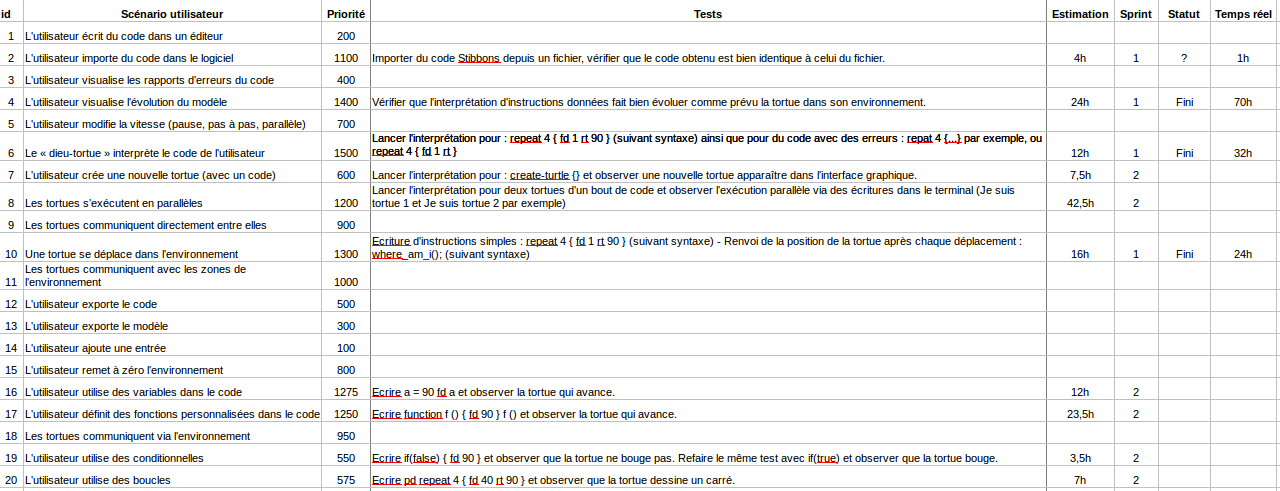
\includegraphics[scale=0.35]{doc/report/uml/backlogv1.png}
\end{figure}
Le backlog est composé de fonctionnalités, qui ont un indice entre 1000 et 0 pour leur importance du rendu final.\\ On écrit aussi une "user-storie" pour chaque fonctionnalité. Cela correspond au test que l'on fait passer au programme pour valider la fonctionnalité.\\
A chaque sprint, on décide des fonctionnalités qu'on ajoute, et du nombre d'heures qu'on estime devoir y passer.\\
Voici pour comparer le backlog lors du début du sprint 4~\ref{backlogsp4} page~\pageref{backlogsp4} :\\
\begin{figure}[h]
\caption{\label{backlogsp4} Backlog sprint 4}
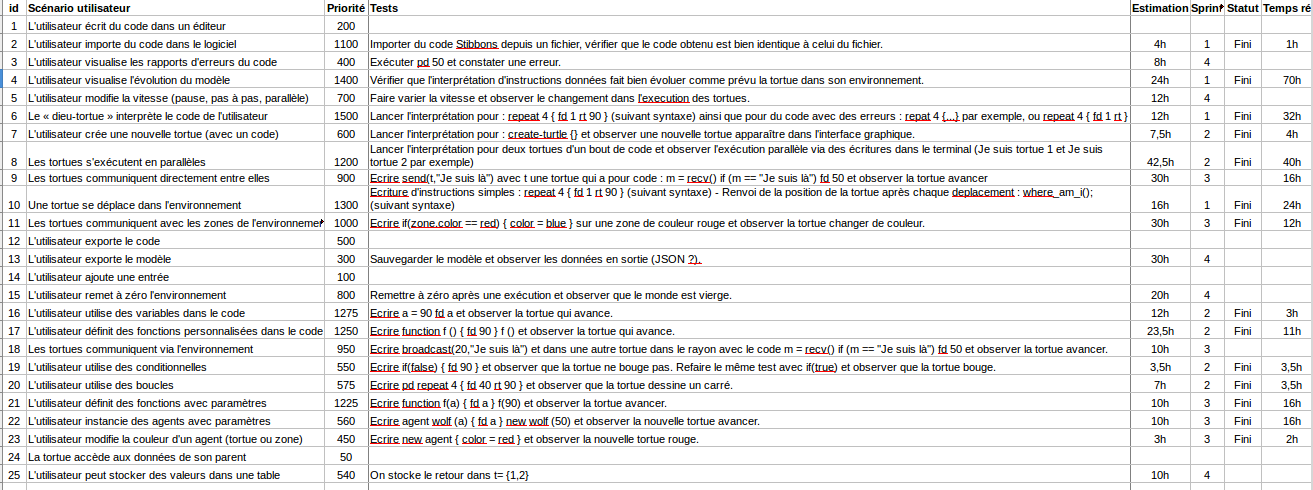
\includegraphics[scale=0.35]{doc/report/uml/backlogsp4.png}
\end{figure}
A la fin d'un sprint, on estime le temps passer sur chaque tâche, on fait le point sur notre avancée dans le projet.\\Ici, on peut voir un ajout de fonctionnalités, le changement de statut des fonctionnalités réalisés, et le temps réel passer à les rendre utilisables.
Globalement, nous étions toujours dans les temps, car nous surestimions certaines tâches, qui s'averait plus facile que prévue.


